\documentclass[border=12pt,tikz]{standalone}
\usepackage[T1]{fontenc}
\usepackage{lmodern}
\usepackage[dvipsnames]{xcolor}
\usetikzlibrary{arrows.meta,positioning,calc,fit,backgrounds}

\definecolor{ink}{HTML}{1A1A1A}
\definecolor{accent}{HTML}{2a78d6}
\definecolor{warn}{HTML}{eb6834}
\definecolor{band}{HTML}{F3F6F9}
\definecolor{accentbg}{HTML}{E9F0F7}
\definecolor{warnbg}{HTML}{FCEFE9}

\hyphenpenalty=10000 \exhyphenpenalty=10000 \tolerance=9999

\begin{document}
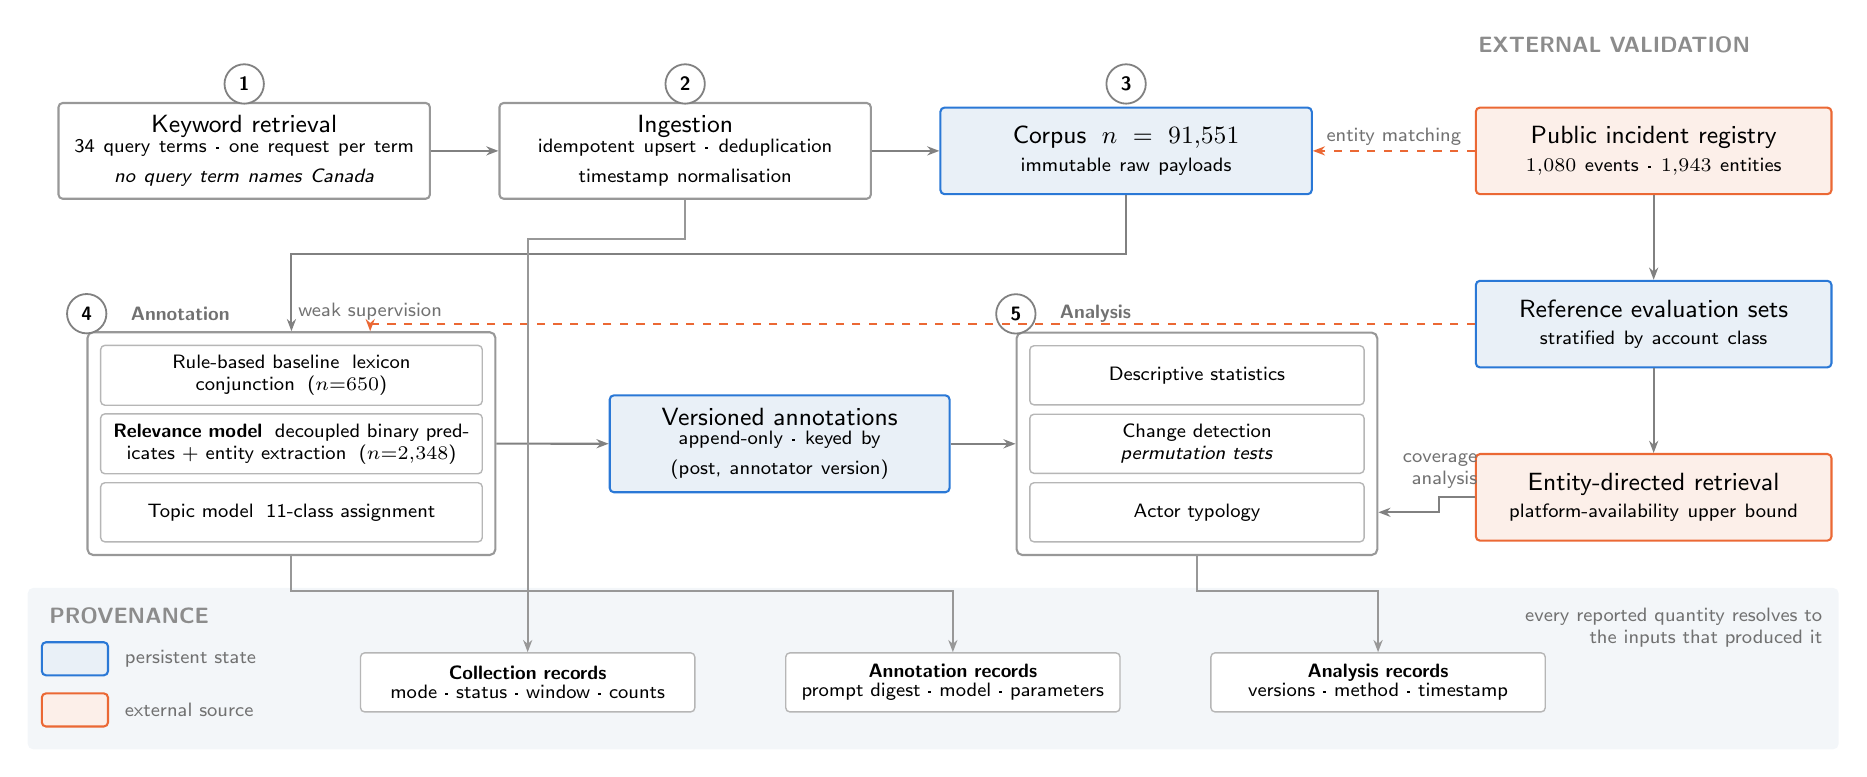
\begin{tikzpicture}[
  font=\sffamily\small, x=1cm, y=1cm,
  stage/.style={draw=ink!45, fill=white, rounded corners=1.5pt, line width=.75pt,
                align=center, inner sep=4.5pt, text width=#1, minimum height=11mm},
  stage/.default=44mm,
  data/.style={stage=#1, draw=accent, fill=accentbg}, data/.default=44mm,
  extn/.style={stage=#1, draw=warn, fill=warnbg},    extn/.default=42mm,
  sub/.style={draw=ink!32, fill=white, rounded corners=1.5pt, line width=.5pt,
              align=center, inner sep=3.5pt, font=\sffamily\scriptsize,
              text width=#1, minimum height=7.5mm}, sub/.default=46mm,
  grp/.style={draw=ink!45, fill=white, rounded corners=2pt, line width=.75pt,
              inner sep=4.5pt},
  num/.style={circle, draw=ink!55, fill=white, line width=.65pt, inner sep=0pt,
              minimum size=5mm, font=\sffamily\scriptsize\bfseries},
  ann/.style={font=\sffamily\scriptsize, text=ink!62, align=center, inner sep=1.5pt},
  ar/.style={-{Stealth[length=4.4pt]}, draw=ink!55, line width=.75pt},
  arw/.style={-{Stealth[length=4.4pt]}, draw=warn, line width=.75pt, dashed},
  hdr/.style={font=\sffamily\footnotesize\bfseries, text=ink!50},
]

%% ---------------- row 1 : acquisition ----------------
\node[stage] (ret) at (0, 0)
  {Keyword retrieval\\[-1pt]{\scriptsize 34 query terms · one request per term\\
   \textit{no query term names Canada}}};
\node[stage] (ing) at (5.6, 0)
  {Ingestion\\[-1pt]{\scriptsize idempotent upsert · deduplication\\timestamp normalisation}};
\node[data]  (cor) at (11.2, 0)
  {Corpus \;$n = 91{,}551$\\[-1pt]{\scriptsize immutable raw payloads}};

\draw[ar] (ret) -- (ing);
\draw[ar] (ing) -- (cor);

%% ---------------- row 2 : annotation, store, analysis ----------------
\node[sub] (a1) at (0.6, -2.85) {Rule-based baseline \;lexicon conjunction \;($n{=}650$)};
\node[sub] (a2) at (0.6, -3.72)
  {\textbf{Relevance model} \;decoupled binary predicates $+$ entity extraction \;($n{=}2{,}348$)};
\node[sub] (a3) at (0.6, -4.59) {Topic model \;11-class assignment};
\begin{scope}[on background layer]\node[grp, fit=(a1)(a2)(a3)] (ann) {};\end{scope}

\node[data=40mm] (out) at (6.8, -3.72)
  {Versioned annotations\\[-1pt]{\scriptsize append-only · keyed by\\(post, annotator version)}};

\node[sub=40mm] (n1) at (12.1, -2.85) {Descriptive statistics};
\node[sub=40mm] (n2) at (12.1, -3.72) {Change detection \;\textit{permutation tests}};
\node[sub=40mm] (n3) at (12.1, -4.59) {Actor typology};
\begin{scope}[on background layer]\node[grp, fit=(n1)(n2)(n3)] (ana) {};\end{scope}

\draw[ar] (ann) -- (out);
\draw[ar] (out) -- (ana);

%% wrap connector: corpus -> annotation
\draw[ar] (cor.south) -- ++(0,-.75) -| (ann.north);

%% stage numbers and group captions
\node[num] at ([yshift=8.5mm]ret.center) {1};
\node[num] at ([yshift=8.5mm]ing.center) {2};
\node[num] at ([yshift=8.5mm]cor.center) {3};
\node[num] at ([shift={(-26mm,16.5mm)}]ann.center) {4};
\node[num] at ([shift={(-23mm,16.5mm)}]ana.center) {5};
\node[ann, anchor=west] at ([shift={(-21mm,16.5mm)}]ann.center) {\textbf{Annotation}};
\node[ann, anchor=west] at ([shift={(-18mm,16.5mm)}]ana.center) {\textbf{Analysis}};

%% ---------------- external validation (right) ----------------
\node[hdr, anchor=west] at (15.55, 1.35) {EXTERNAL VALIDATION};
\node[extn] (src) at (17.9, 0)
  {Public incident registry\\[-1pt]{\scriptsize $1{,}080$ events · $1{,}943$ entities}};
\node[data=42mm] (ev) at (17.9, -2.2)
  {Reference evaluation sets\\[-1pt]{\scriptsize stratified by account class}};
\node[extn] (edr) at (17.9, -4.4)
  {Entity-directed retrieval\\[-1pt]{\scriptsize platform-availability upper bound}};

\draw[ar] (src) -- (ev);
\draw[ar] (ev) -- (edr);
\draw[arw] (src.west) -- node[ann, above, pos=.5]{entity matching} (cor.east);
\draw[arw] (ev.west)  -- ++(-.7,0) -| node[ann, above, pos=.62]{weak supervision} ([xshift=10mm]ann.north);
\draw[ar]  (edr.west) -- ++(-.45,0) |- ([yshift=-8.7mm]ana.east);

\node[ann, anchor=south east, align=right] at (15.72, -4.35) {coverage\\analysis};

%% ---------------- provenance band (bottom) ----------------
\begin{scope}[on background layer]
  \node[fill=band, rounded corners=2pt, inner sep=0pt,
        fit={(-2.75,-7.6) (20.25,-5.55)}] {};
\end{scope}
\node[hdr, anchor=west] at (-2.6, -5.9) {PROVENANCE};
\node[sub=40mm] (p1) at (3.6, -6.75)
  {\textbf{Collection records}\\[-1pt]mode · status · window · counts};
\node[sub=40mm] (p2) at (9.0, -6.75)
  {\textbf{Annotation records}\\[-1pt]prompt digest · model · parameters};
\node[sub=40mm] (p3) at (14.4, -6.75)
  {\textbf{Analysis records}\\[-1pt]versions · method · timestamp};
\node[ann, anchor=east, text width=42mm, align=right] at (20.1, -6.05)
  {every reported quantity resolves to\\the inputs that produced it};

\draw[ar, draw=ink!45] (ing.south) -- ++(0,-.5) -| (p1.north);
\draw[ar, draw=ink!45] (ann.south) -- ++(0,-.45) -| (p2.north);
\draw[ar, draw=ink!45] (ana.south) -- ++(0,-.45) -| (p3.north);

%% ---------------- legend ----------------
\node[data=7mm, minimum height=4.2mm, inner sep=2pt] (lg1) at (-2.15, -6.45) {};
\node[ann, anchor=west] at ([xshift=1.4mm]lg1.east) {persistent state};
\node[extn=7mm, minimum height=4.2mm, inner sep=2pt] (lg2) at (-2.15, -7.1) {};
\node[ann, anchor=west] at ([xshift=1.4mm]lg2.east) {external source};

\end{tikzpicture}
\end{document}
